\chapter{BACKGROUND}
\label{background}
%Some mathematical techniques which are used to solve the problems in thesis are introduced in this chapter.

In the past few years, game theory has been extensively applied to problems in communication and networking~\cite{Neel06analysisand, Wang_gtc_crn_survey_2010}.
Game theory is a powerful mathematical tool for studying, modelling and analysing the interaction among rational decision makers which have conflicting objectives.
When the network entities are seen as rational, game theory can be used to predict and guide the behaviour of them, and predict the outcome of the system with respect to certain metrics.
In contrary to game theory where players agree on an equilibrium via autonomous behaviours, optimization problem, which attempts to optimize the welfare of either one equipment or whole network, is usually conducted on a single decision maker.
In the following, we introduce some basics of game theory and optimization.





\section{Algorithmic Game Theory}


Game theoretic models are used to understand many challenging problems in communication systems, such as resource allocation, topology control, routing, security and so on. 
%In recent years, game theory attracts people attention into apply it in communication systems.
There are several reasons to apply game theory in communication systems.
\begin{itemize}
\item Communication equipments are rational.
Although current communication equipments involve only a little artificial intelligence, they are supposed to be manufactured and operate based on standards to fulfil certain functions, but selfish behaviour may appear on certain individual equipments to achieve advantages over their peers~\cite{game_for_communication_01}.

In communication system, a device is programmed to maximize or minimize the expected utility, which is perfectly rational.
For instance, Wi-Fi equipments are manufactured complying the IEEE 802.11 standards.
But it is possible that certain manufacturers or the personal who uses the Wi-Fi system (we use station in the following) manipulate certain parameters to achieve performance advantage over other stations in the network.
When all the stations in one network are supposed to run distributed coordination function (\gls{DCF}), \ie the station must wait a random period of time, which is called contention window (\gls{CW}), before accessing the media when it senses the media to be busy, a certain selfish station may not choose to wait and is keen on sensing media.
The selfish behaviour causes more collisions for other stations, and possibly results in poor performance in the network.
%In this case, the access point finds more packets coming from that selfish user, but is unaware of its selfishness and has no means to adjust or punish this selfish user.
In this case, game theory facilitates the network operator to issue rules to make the selfish behaviour unprofitable, or it helps to analyse how much the impact caused by the selfish stations.
% can tell the access point or network operator the impact caused by the selfish systems, and possibly 

\item Game theory is effective to solve networking problems.
Algorithms can be retrieved from the analysis of a problem under the game theoretical framework.
In the same example of media access in IEEE 802.11 DCF mentioned in previous item, if stations are allowed to modify the length of contention window, each station will adjust its contention window to obtain the best performance.
\cite{contentiongame_07} shows as long as each station greedily updates its CW to maximize certain utility, after certain time it will stop to do so as the current CW is the best as to the performance.
In the case, the best response becomes a algorithm for Wi-Fi systems.
%They interact with each other and update their contention windows, when they reach Nash Equilibrium state, no system has motivation to change its contention window any more.
%
Besides, outcome from game theory is robust~\cite{Han:2008:RAW:1457343}.
As to optimization, when the information is not accurate or adequate enough, or the optimization itself is difficult to solve, the optimized results can be far from global optimality.
Game theory based on the local information, which is easy to obtain, usually leads to Nash equilibrium (\gls{NE}), which is usually sub optimal.


\item Game theory is suitable to apply in cognitive radio network because of the properties of CRN.
Firstly, only local information is needed, thus game theory is naturally suitable for designing distributed solutions for cognitive radio networks.
Distributed solutions doesn't rely on centralized controller, and each user in the network adopts certain action as response to the other users or environment, this falls in the scope of game theory.
%
Secondly, combinatorial nature of communication problems makes game theory as one of a few choices~\cite{Han:2008:RAW:1457343}.
Many problems in wireless communication involve integer variables, \ie channel assignment, selection of modulation levels or channel coding.
It is always challenging to solve combinatorial optimization problems, whereas game theory is natural to describe it in a discrete form.

\end{itemize}




 

%\todo[inline]{expand: Introduction of game theory...}
\subsection{Basics of Game}
%Game theory is established by Nash in xxxx, and is applied in network communication since xxx
In this section, we give a brief introduction of game theory and congestion game which is applied to solve problems in our thesis.
The notations used in this thesis comply with~\cite{agt_book}.


%\subsubsection*{Strategic Game}

A strategic game can be represented as a tuple $\Gamma = (\mathcal{N}, (\mathcal{S}_i)_{i \in \mathcal{N}}, (u_i)_{i\in \mathcal{N}})$, where 
\begin{itemize}
\item $\mathcal{N}$ is a finite set of players.
\item $\mathcal{S}_i$ is player $i$' set of strategies.
Player $i$ selects one strategy $s_i\in \mathcal{S}_i$ at one time to play the game.
\item $\mathcal{S} = \mathcal{S}_1\times\cdots\times \mathcal{S}_n$ is the set of states, which denotes all the possible ways that players may pick strategies.

\item $s=(s_i,\cdots,s_n)$ is vector of strategies and also is called as one strategy profile, which represents an instance of all players' choices.
There is $s\in \mathcal{S}$.

\item The vector of strategies of opponents of player $i$ is expressed as $s_{-i}$, and the corresponding strategy profile can be shown as $s=\{s_i, s_{-i}\}$.
$u_i(s) = u_i(s_i, s_{-i})$ is the player $i$' outcome in strategy profile $s$.

\item $u_i:\sqcap_{i\in \mathcal{N}}\mathcal{S}_i\rightarrow \mathbb{R} $ is the utility function of player $i$.
%$\sum=\sqcap_{i\in \mathcal{N}}\sum_i$ is the set of states of the game, which denotes all the possible ways that players may pick strategies.
$\mathcal{S}_{-i}=\sqcap_{i\in \mathcal{N}\setminus \{i\}}\mathcal{S}_i$ is the set of states of all the other players except for player $i$.
As to each player $i$, its outcome is decided by its choice on strategy $s_i\in \mathcal{S}_i$, and is also dependant on the choices of other players $s_{-i}\in \mathcal{S}_{-i}$.
Utility can also be denoted as $u_i(s)$ or $u_i(s_i,s_{-i})$ to stress that the outcome is made based on all players' strategies.


Utility function is very important to specify a game, as it gives players preferences on the outcomes with respect to all strategy vectors $\mathcal{S}$.
The value of the utility can be regarded as payoffs or costs depending on concrete scenarios.
The sum of costs and payoffs are zero, and they can be used interchangeably.
\end{itemize}




When we want to use game theory to analyse a problem in CRN, it is critical to formulate appropriate components of the problem into corresponding elements of a game.
The commonly used formulation is summarized in Table~\ref{game_crn_component}.

\begin{table}
\centering
\begin{tabular}{|c|C{7cm}|}
\hline 
Elements of a game & Components of one CRN \\ 
\hline 
Player $\mathcal{N}$ & secondary users \\ 
\hline 
Strategies for player $i$, $\mathcal{S}_i$  & working channels, transmission power, modulation, etc. \\ 
\hline 
Utility of player $i$, $u_i$ & performance in respect of SINR, throughput, etc. \\ 
\hline 
\end{tabular} 
\caption{Components of problems in CRN and corresponding elements in game}
\label{game_crn_component}
\end{table}




\subsection{Basic Solution Concepts}
In this section, we will introduce some basic solution concepts, some of them are used in this thesis.
\subsubsection*{Dominant Strategy Solution}
In some games, each player has a unique best strategy, which is independent of the strategies chosen by the other players, then we say a game of this kind has a dominant strategy solution.
The mathematical expression is, a strategy vector $s\in \mathcal{S}$ is a dominant strategy, if for each player $i$ and each alternate strategy $s'\in \mathcal{S}$, there is, 
 \[ u_i(s_i, s_{-i}') \geq u_i(s_i', s_{-i}')\]

Note that a dominant strategy solution may not give an optimal payoff to any of the players.
This is the case in \textit{prisoner's dilemma}, which is one of the most well known and well studied games.
To confess is the dominant solution for both prisoners, which brings them longer time behind bars than that when both of them keep silent\footnote{Prisoner's dilemma can be found in almost all the game theory textbooks, thus omitted in this thesis.}.
Only a few games have dominant strategy, and mechanism design~\cite{Design_Mechanisms_1973} is developed to design games which have dominate strategy, and these dominate strategies lead to desirable outcome.



\subsubsection*{Nash Equilibrium}
A desirable solution of games is the one that players choose strategy in accordance with their incentives, minimizing their own cost or maximizing their own payoff.
Nash equilibrium successfully captures this property, and is the most discussed and pursued solution concept in game theory~\ref{game_crn_component}.

A strategy vector $s\in S$ is a \textit{Nash equilibrium} if for any player $i$ and each alternate strategy $s_i'$, there is
 \[ u_i(s_i, s_{-i}) \geq u_i(s_i', s_{-i})\]
This means for any player in NE state, no unilateral deviation from its current strategy is more profitable.
This also implies that, NE is self enforcing that once players agree on this solution, it is the best interest for every player to stick to its current strategy.

A dominant strategy is a Nash equilibrium, and is also the unique NE, but a NE is not necessarily a dominant strategy.
There may be multiple NEs in one game, and NE may not be optimal for players. 
In prisoner dilemma, the dominating strategy is NE but is obviously not the optimal.
Games with finite number of players and strategy set are guaranteed to have NE, whereas, games with an infinite number of players, or games with a finite number of players but they can access to an infinite strategy set may not have NE~\cite{agt_book}.


Being not unique and possibly sub-optimal, NE is still applied in extremely diverse applications due to the reasons in the beginning of this section.
Thus, when pursue NE as solution, people should answer the following questions,
The first question is, what is the gap between NE and global optimal?
This can be partially answered by \textit{price of anarchy (\gls{PoA})}, the ratio between the worst-case Nash equilibrium to the optimality is used to denote the quality of the solution.

Nash equilibrium is an appealing conception, but it doesn't tell how to reach this state.
Hence, it is important to find an efficient algorithm to reach the equilibrium.
Theoretical scientists tell \textit{finding a Nash equilibrium} problem is a combinatorial problem ans is often very difficult (Chapter 2, \cite{agt_book}).
Moreover, the notion of \textit{NP-completeness} is not an appropriate concept of complexity for \textit{finding a Nash equilibrium} problem as NE always exists, in stead.
Nevertheless, in some games, because of the special strategy space structure, or players' special behaviours, efficient algorithm to reach NE exists.





%Nash equilibrium is a conceptual tool and a prediction about the rational strategic behaviour by agents in situations of conflict, hence, it carries great importance to know how much computational effort needed to compute NE.



\subsubsection*{Pareto Equilibrium}
%There exists other equilibrium conceptions. \ie Pareto Equilibrium . 
\textit{Pareto equilibrium} (\gls{PE}) is a subset of NE, PE is an action profile $\bar{s}$ such that there does not exist profile $s$ with $u_i(s)\leq u_i(\bar{s})$ for each $i\in N$, and meanwhile $u_i(s)< u_i(\bar{s})$ for at least one $i\in N$.
PE is the necessary condition of the global optimality and accordingly is more favoured, but its application in communication system is much less than NE because it is not easy to obtain PE.


\subsubsection*{Pure NE and Mixed NE}
In the aforementioned games, players deterministically play their chosen strategies and don't involve randomized strategies, then the achieved NE is called pure NE. 
When players play a game with certain randomization on strategies, and aim to maximize their expected payoff, we call the resulted NE as mixed NE.
As to mixed NE, the action of a player is to choose certain strategies according to a vector of probabilities.
In this thesis, we only consider pure NE, as players deterministically play a certain strategy, and the corresponding network components stick to certain operation instead to switch among several different operations based on a vector of probabilities.

Other solutions include correlated equilibrium, which also involves probability distribution over strategy vectors.


%Unlucky, the computation of NE is usually a combinatorial optimization problem (chapter 2)~\cite{}.
% but in some special cases, 

%\subsubsection*{Different Games in Nutshell}


\subsubsection*{Individual Optimization and Game}
As to a player in a game, when its utility $u_i$ is function of its strategy $s_i$, and not the strategies chosen by all $n$ players, then the maximization of its payoff or minimization of its cost becomes an optimization problem, and the game has $n$ such optimization problems in total.
Whereas as to a game, the payoff or cost of each player depends on both $s_i$ and $s_{-i}$, both its own strategy and the strategies chosen by all other players.






\subsection{Congestion Game}
In accordance with~\cite{Voecking06congestiongames}, congestion game is a game where players simultaneously allocate sets of resources to minimize its utility, and the cost of a resource is a function of congestion, which is the number of players choosing the resource.
Congestion game can be formulated from many problems in realistic world, \eg minimisation of commuting time on the road for commuters, minimization of energy consumption in mobile cloud computing system~\cite{game_cloudcomputing_energy12}.



%\subsubsection*{Potential Game}
%A potential game is a tuple $\lambda=(\mathcal{N},(\sum_i)_{i \in \mathcal{N}},(u_i)_{i\in \mathcal{N}})$, which satisfies the following, if there exists a function $\phi: \sum\rightarrow \mathbb{R}$, such that for every $i\in \mathcal{N}$, for every $s_{-i}\in \sum_{-i}$, and every $s_i, s_i'\in \sum_i$:
% \[ u_i(s_i, s_{-i})-u_i(s_i', s_{-i}) = \phi_i(s_i, s_{-i})-\phi_i(s_i', s_{-i})\]
%It is easy to see that the design of function $\phi$ is the key point to form a potential game.


%\subsubsection*{Congestion Game}

%Congestion game is a special type of potential game, which has extra conditions, but also yield favourable characteristics.

%In congestion game, player pays for the resources it occupies.
%Particularly, the payment for one resource is monotonically increasing with the \textit{number} of players occupying that resource, and each player tries to minimize its payment~\footnote{Another way to describe congestion game: player gets benefit by using a certain resource, the benefit is monotonically decreasing with the number of players on that resource, each player tries to maximize its welfare}. 



Now we give the formal definition of congestion game.
A congestion game \cite{Rosenthal}\cite{Voecking06congestiongames} can be expressed by a tuple $\lambda=(\mathcal{N},\mathcal{R},(\mathcal{S}_i)_{i \in \mathcal{N}},(g_r)_{r\in \mathcal{R}})$, where $\mathcal{N}=\left\{1,\ldots,N\right\}$ denotes the set of players (each each is labeled with a unique index number), $\mathcal{R}=\left\{1,\ldots,m\right\}$ the set of resources, $\Sigma_{i\in\mathcal{N}} \subseteq 2^{\mathcal{R}}$ is the strategy space of player $i$. 
Under strategy profile $s=(s_1,s_2,\cdots s_N)$, player $i$ chooses strategy $s_i\in \mathcal{S}_i$, and the total number of users using resource $r$ is $n_r(s)=|\{i\mid r\in s_i\}|$. 
The cost $g_r: \mathbb{N}\rightarrow \mathbb{Z}$ is a function of the number of users for resource $r$, $g_r^i=\sum_{r\in s_i} g_r(n_r(s))$. 
In our paper, $g_r^i$ is referred as congestion of a game.
Congestion game has good property that Nash equilibrium are guaranteed after finite improvement, thus it is an attractive game model which describes the problem where participants compete for limited resources in a non-cooperative manner.


\subsubsection*{Example: Server Matching}
We introduce an exemplary congestion game \textit{server matching}~\cite{kothari:congestion_serverMatching} to illustrate the extensive application of game theory in communication systems.
Consider a couple of self-interested clients and servers as shown in Figure~\ref{server_sharing}.
Each client is allowed to access one server.
The latency of one server increases with the \textit{number of clients} attached to it.
When clients try to choose one server which has the shortest latency, a congestion game is formed.
\begin{figure}[h!]
  \centering
  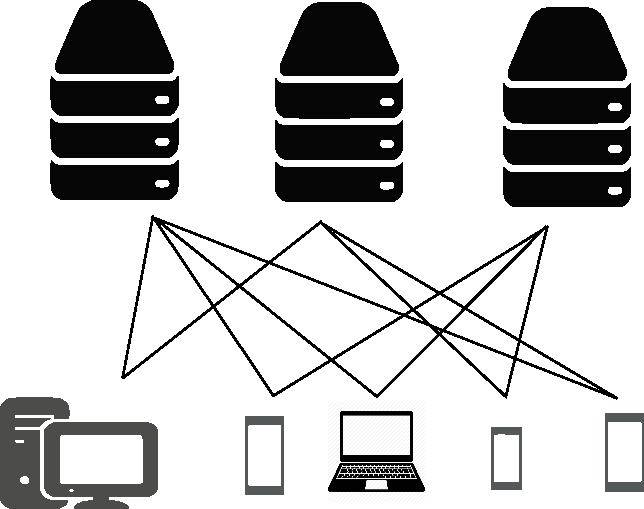
\includegraphics[width=0.6\linewidth]{server_sharing.pdf}
  \caption{An example server matching, one server is possible strategy of the client at the other end of the connecting line}
\label{server_sharing}
\end{figure}

More formally, this corresponding congestion game is composed of players (the self-interested clients) and resources (servers), where players are allowed to choose certain resources to use. 
There is cost (latency) generated on a resource for the player whenever the player uses that resource, and the cost is monotonic increasing with the number of players using it. 
As congestion game permits convergence when every player always adopts the strategy which leads to better performance, thus in server matching problem, when clients choose a permissible server because of smaller predicted latency, then after finite number of choices, no client has motivation to switch any more.
%If every player greedily searches the allowed resources to decrease its cost, the dynamics will cease in Nash equilibrium, where no player has motivation to adopt a new set of resources unilaterally. 

Congestion game can also be used to model many other problems in internet-centric applications or cloud computing, where self-interested clients compete for the centralized resources and meanwhile interact with each other.
For example, server selection is involved in distributed computing platforms~\cite{Cloud_Computing_2010}, or users downloading files from cloud, etc.






\subsubsection*{Convergence Time Towards Nash Equilibrium}
As to the convergence of congestion game, there is a proposition~\cite{Voecking06congestiongames} saying, for every congestion game, every sequence of improvement steps is finite.
In the following, we introduce the sketch of the proof of the proposition, as the proving procedure also reveal the number of improvement steps to reach Nash Equilibrium.

We firstly need to introduce Rosenthal's potential function $\phi(s):\rightarrow Z$, where $s$ is the strategy profile of all the players, $s = s_1\times s_2\times\cdots\times s_N$:
\begin{equation}
\label{4}
\begin{split}
\phi(s) 
& =\sum\limits^{}_{r\in \mathcal{R}} \sum\limits^{n_r(s)}_{i=1} g_r(i)\\
& =\sum\limits_{i\in \mathcal{N}} \sum\limits^{}_{r\in s_i} g_r(n_r^i(s))\\
\end{split}
\end{equation}
$n_r^i(s)$ is the number of players using resource $r$, whose indices are smaller than or equal to $i$, \ie from $\{1,\cdots,i\}$. 
In the part after the second equality sign, $\sum\limits^{}_{r\in s_i} g_r(n_r^i(s))$ is a virtual value or cost that player $i$ have when assuming the resource $r$ is not used by players whose indices are greater than $i$.
%Note that the potential is \textit{not} the sum of congestions experienced by every user. 

The intuitive interpretation of the virtual cost is, according to~\cite{Voecking06congestiongames}, the cost of each player for choosing the strategy when it is inserted into the game.
Let us assume player $N$ is the last player to be inserted into the game, then $\sum\limits^{}_{r\in s_N} g_r(n_r^N(s))$ equals to the real cost that player $n$ takes.
When player $N$ can decrease its cost by switching to another strategy by an unilateral move, then $\sum\limits^{}_{r\in s_N} g_r(n_r^N(s))$ and its potential decrease by the same amount.
As the potential can be calculated by inserting the players with any sequence, each player will have the same property with play $N$, as we just discussed.

In summery, the change of the potential caused by one player's unilateral move from $s_i$ to $s_i'$ is equivalent to the change of gain (or loss) of that player.
\begin{equation}
\label{5}
\varDelta \phi(s_i \rightarrow s_i') = g^i(s',s_{-i}) - g^i(s,s_{-i})
\end{equation}
$s_{-i}$ is the strategy profile for all players except for $i$.
Thus the potential decreases with the update of players monotonically during the convergence process.
Most importantly, as the potential of a congestion game is bounded by some finite quantity, and every improvement made by player decreases it, the length of any sequence of improvement steps is also finite.



%As every congestion game is a potential game, and the total potential is finite, thus the number of improvements is upper-bounded by $2\cdot\sum\limits^{}_{r\in \mathcal{R}} \sum\limits^{n_r(\sigma)}_{i=1} g_r(i)$ \cite{Voecking06congestiongames}.

%\section{Application of congestion game in the design of decentralised algorithm}
%\todo[inline]{expand: the application of potential game in CRN}



\section{Optimization}
As discussed in Chapter~\ref{INTRODUCTION}, the available radio resources such as spectrum and transmission power are very limited, meanwhile, new services raise great requirements for these resources.
Resource allocation and its optimization are able to accommodate the needs.
Various optimization problems are formulated to improve radio resource usage in CRN~\cite{cacao_ca_2011, fuzzy_decision_09, resourceAllocation_imperfectSensing_2012}.
Optimization can be conducted from either global view or individual perspective.

Many wireless resource allocation problems are formulated as constrained optimization problems.
Table~\ref{opt_table} shows the commonly used parameters, objectives and constraints in optimization problems of wireless communication.
A Part of the contents in Table~\ref{opt_table} refers \cite{Han:2008:RAW:1457343}.

\begin{table}
\begin{tabular}{|C{2.2cm}|C{3.8cm} | C{3.5cm} | C{3.7cm}|}
\hline 
 & Parametres & Optimization goals & Constraints \\ 
\hline 
Application layer & source-coding rate, buffer priority, packet arrival rate & minimal delay & base layer transmission, strict delay requirement \\ 
\hline 
Network layer & routing path & end to end delay/throughput & maximal hops, security concerns \\ 
\hline 
MAC layer & transmission frequency, transmission priorities & maximal overall throughput, minimal buffer overflow probability & contentions, time/frequency slot \\ 
\hline
Physical layer & transmission power, modulation, channel coding rate & minimal over power consumption, maximal throughput, minimal BER & maximal transmission power, caused interference on licensed users, available channel coding rate \\ 
\hline
\end{tabular} 
\caption{Optimization problem of cognitive radio networks}
\label{opt_table} 
\end{table}

The solutions to optimization problems can be categorized with their properties, \ie convex, linear, integer, or non-convex non-linear, etc.
In this thesis, we make use of solvers, \ie Lindo, Gurobi, to solve the formulated optimization problems.


%Optimization outputs the results with the global information.
%Optimization is implemented on one entity, thus it is naturally suitable in centralized scheme.
